\begin{flushright}
	\BLOCK{ if tags.name }
	\textbf{\VAR{tags.name}}
	\BLOCK{ endif }

	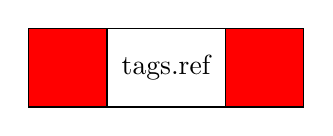
\begin{tikzpicture}
	\draw [fill=red] (0, 0) rectangle (1, 1);
	\draw [fill=white] (1, 0) rectangle (2.5, 1) node[pos=.5] { \VAR{tags.ref} };
	\draw [fill=red] (2.5, 0) rectangle (3.5, 1);
	\end{tikzpicture}
	
	\VAR{tags.cai_scale}
	\BLOCK{ if tags.old_ref }
	(\VAR{tags.old_ref}})
	\BLOCK{ endif }
	
	\BLOCK{ if tags.rwnname }
	\VAR{tags.rwnname}
	\BLOCK{ endif }
	
	\BLOCK{ if tags.refREI }
	\VAR{tags.refREI}
	\BLOCK{ endif }	
	
	\BLOCK{ if tags.network == 'lwn' }
	\tiny{Sentiero locale}
	\BLOCK{ elif tags.network == 'rwn' }
	\tiny{Sentiero regionale}
	\BLOCK{ elif tags.network == 'nwn' }
	\tiny{Sentiero nazionale}
	\BLOCK{ elif tags.network == 'iwn' }
	\tiny{Sentiero internazionale}
	\BLOCK{ endif }
\end{flushright}
\textit{
\BLOCK{ if tags.from }
\VAR{tags.from} 
\BLOCK{ endif }
\BLOCK{ if tags.to }
- \VAR{tags.to}
\BLOCK{ endif }
}
\bigskip

\section*{Informazioni sul sentiero}
\begin{tabular}{lp{0.8\textwidth}}
	\BLOCK{ if tags.distance }
	Distanza: & \VAR{tags.distance} Km \\
	\BLOCK{ else }
	Distanza: & \\
	\BLOCK{ endif }
	Durata andata: & \VAR{tags.durationforward} \\
	Durata ritorno: & \VAR{tags.durationbackward} \\
	\BLOCK{ if tags.ascent }
	Dislivello positivo & \VAR{tags.ascent} m \\
	\BLOCK{ else }
	Dislivello positivo &  \\
	\BLOCK{ endif }
	\BLOCK{ if tags.descent }
	Dislivello negativo & \VAR{tags.descent} m \\
	\BLOCK{ else }
	Dislivello negativo & \\
	\BLOCK{ endif }	
	\BLOCK{ if tags.descriptionit }
	Descrizione: &  \VAR{tags.descriptionit} \\
	\BLOCK{ else }
	Descrizione: &  \VAR{tags.description} \\
	\BLOCK{ endif }
	\BLOCK{ if tags.roundtrip == 'yes' }
	Sentiero circolare: &  si \\
	\BLOCK{ else }
	Sentiero circolare: &  no \\
	\BLOCK{ endif }
\end{tabular}

\section*{Informazioni mantenimento}
\begin{tabular}{lp{0.8\textwidth}}
	Sorgente: & \VAR{tags.source} \\
	Data rilievo: & \VAR{tags.sourveydate} \\
	Operatore: & \VAR{tags.operator} \\
	Stato: & \VAR{tags.state} \\
	\BLOCK{ if tags.maintenanceit }
	Mantenimento: &  \VAR{tags.maintenanceit} \\
	\BLOCK{ else }
	Mantenimento: &  \VAR{tags.maintenance} \\
	\BLOCK{ endif }
	\BLOCK{ if tags.noteit }
	Note: &  \VAR{tags.noteit} \\
	\BLOCK{ else }
	Note: &  \VAR{tags.note} \\
	\BLOCK{ endif }
\end{tabular}

\vspace*{\fill}
\begin{flushright}
	\BLOCK{ if tags.website }
	\url{\VAR{tags.website}}
	\BLOCK{ endif }
	\url{https://www.openstreetmap.org/relation/\VAR{tags.id}}	
\end{flushright}